\documentclass[9pt,twocolumn,twoside]{../../styles/osajnl}
\usepackage{fancyvrb}
\journal{i524} 

\title{Analysis Of People Relationship Using Word2Vec on Wiki Data}

\author[1,*]{Abhishek Gupta}
\author[1, **]{Avadhoot Agasti}

\affil[1]{School of Informatics and Computing, Bloomington, IN 47408, U.S.A.}

\affil[*]{Corresponding authors: abhigupt@iu.edu}
\affil[**]{Corresponding authors: aagasti@iu.edu}

\dates{project-1: Data mining for a wiki url , \today}

\ociscodes{Cloud, I524}

% replace this with your url in github/gitlab
\doi{\url{https://github.com/cloudmesh/sp17-i524/blob/master/project/S17-IR-P005/report/report.pdf}}

\begin{abstract}
Given a wiki URL of a person, find out his details like School, Spouse, Coaches, language, alma-meter etc Typically, the wiki page has all this information available but in the free form text. We need to converting it into structured data format so that it can help us analyze the people, from the networks etc We can create a network by navigating the people mentioned in the wiki page. 
\end{abstract}

\setboolean{displaycopyright}{true}


\begin{document}

\maketitle

\tableofcontents

\section{Introduction}

Use spark \cite{www-spark-python} to load the wiki data and create word vectors. Train it using spark ML  \cite{www-sparkml} and then use the model for analytics and prediction. The training set will use Word2Vec. Word2vec \cite{www-word2vec} is a group of related models that are used to produce word embeddings. Word2Vec is used to analyze the linguistic context of the words. In this project, we created Word2vec model using Wikipedia data. Our focus is people and organization names occurring in the Wikipedia data and to see if Word2vec can be used to understand relationship between people. Typically Wikipedia page for people and celebraties contain the entire family and friends, colleagues information. Our idea is to use Word2vec to see if using a smaller training set of known relationships whether we can derive similar relationship for anyone who has presence on Wikipedia. This mechanism can be then used to convert the data hidden in textual format to more structured data. 

\begin{center}
 \begin{tabular}{||c l||} 
 \hline
 Technology Name & Purpose  \\ [0.5ex] 
 \hline\hline
 spark \cite{www-spark-python} & data analysis  \\
 \hline
 sparkML \cite{www-sparkml} & machine learning  \\
 \hline
 python \cite{www-spark-python} & development \\
 \hline
 ansible \cite{www-ansible} & automated deployment \\
 \hline
 collectd \cite{www-collectd} & statistics collection for benchmarking \\
 \hline
\end{tabular}
\end{center}

\section{Plan}
Following table gives a breakdown of tasks in order to complete the project. Assuming week1 starts after submission of the proposal. These work items are high level breakdown on the tasks and may changes if needed.

\begin{center}
\begin{tabular}{ |c|l|c| } 
 \hline
Week & Work Item & Status \\
\hline
week1 & Basic POC of Word2Vec using Python  & planned \\ 
week2 & Scripts to download Wiki data & planned \\ 
week3 & Word2Vec Spark program & planned \\ 
week4 & Training and measuring accuracy & planned \\ 
week5 &  Ansible Deployment script for Spark & planned \\ 
week6 & Deployment and test on 2 clouds & planned \\ 
week7 & Performance measurement  & planned \\ 
week8 & Report Creation(parallel) & planned \\ 
 \hline
\end{tabular}
\end{center}

%\section{Design}
%TBD
\section{Design} \label{designsection}

\begin{figure}[htbp]
\centering
\fbox{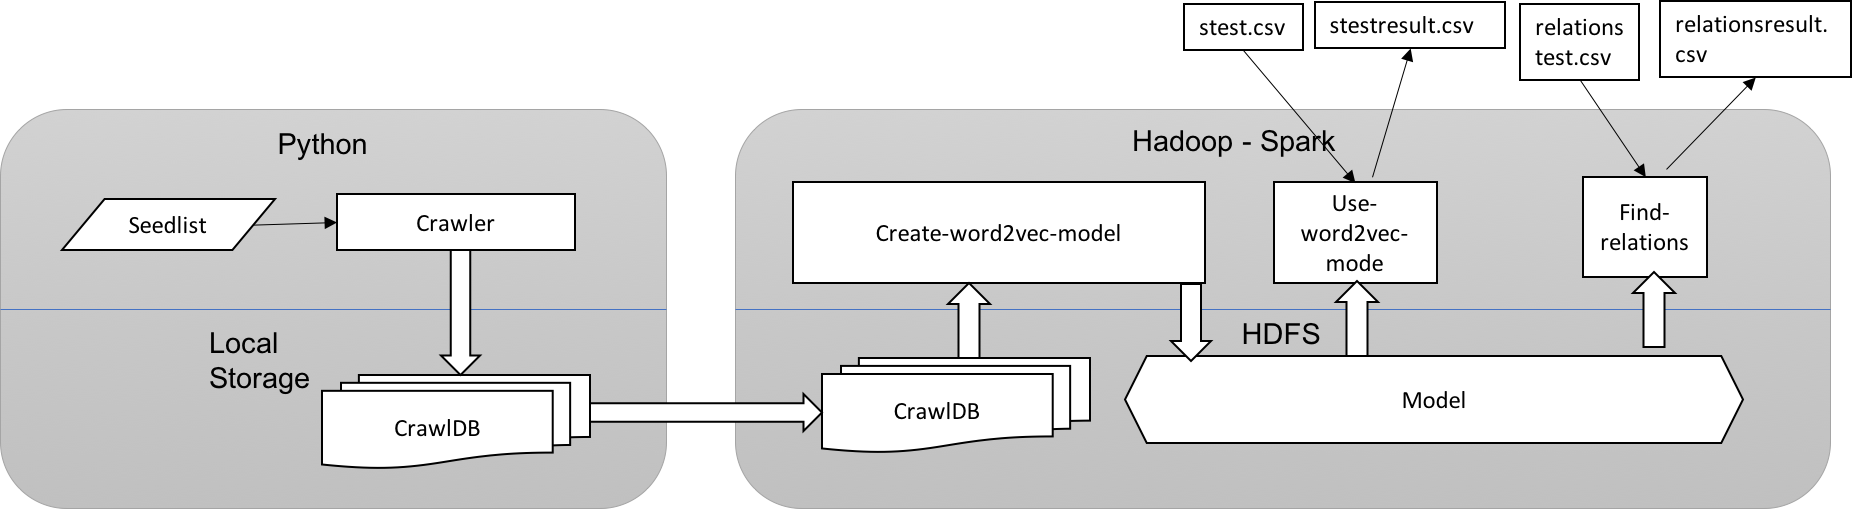
\includegraphics[width=\linewidth]{images/datapipeline.png}}
\caption{Data Pipeline.}
\label{fig:datapipeline}
\end{figure}

Figure \ref{fig:datapipeline} shows the overall data pipeline for the
project. The data pipeline has three important stages:
\begin{itemize}
\item Crawler: Crawler runs in batch mode on a standalone machine. It can
download wikipedia data as explained in section \ref{crawlersection}. Crawler
 creates CrawlDB which is a collection of text files. This crawler can be
 replaced or augmented with any web-crawler which can download or create the
 text files.

\item create-word2vec-model: This component is responsible for creating the
word2vec model for the text files in the CrawlDB. This model runs on Spark
and stores the model on HDFS. Section \ref{createmodelsection} describes this
 component in detail.

\item use-word2vec-model and find-relations: These two components use the
precreated word2vec model to find synonym of a word or find the relationships.
Section \ref{usemodel} describes these components in detail.
\end{itemize}

\subsection{Crawler} \label{crawlersection}
The Crawler component is useful to download the data from web. We implemented
 a simple crawler using Python which can deep traverse the wikipedia pages
 and download the text from it. In our crawler implementation, a user can
 specify the seed pages from wikipedia. User can also specify the maximum
 number of pages that are required to be downloaded. The crawler first
 downloads all the pages specified in the seedlist. It then extract the links
  from each wikipedia page and puts it in a queue which is internally
  maintained by the crawler. The crawler then downloads the the linked pages.
   Since this logic is implemented in recursive manner, the crawler can
   potentially download all the wikipedia pages which can be reached from the
   pages in the seedlist.

    We followed the seedlist based crawler approach so that we can retrieve
    domain specific web pages. A well chosen seedlist can fetch large number
    of relevant web pages.

 Figure \ref{fig:crawleralgo} is the flowchart of the crawler implementation.
\begin{figure}[htbp]
\centering
\fbox{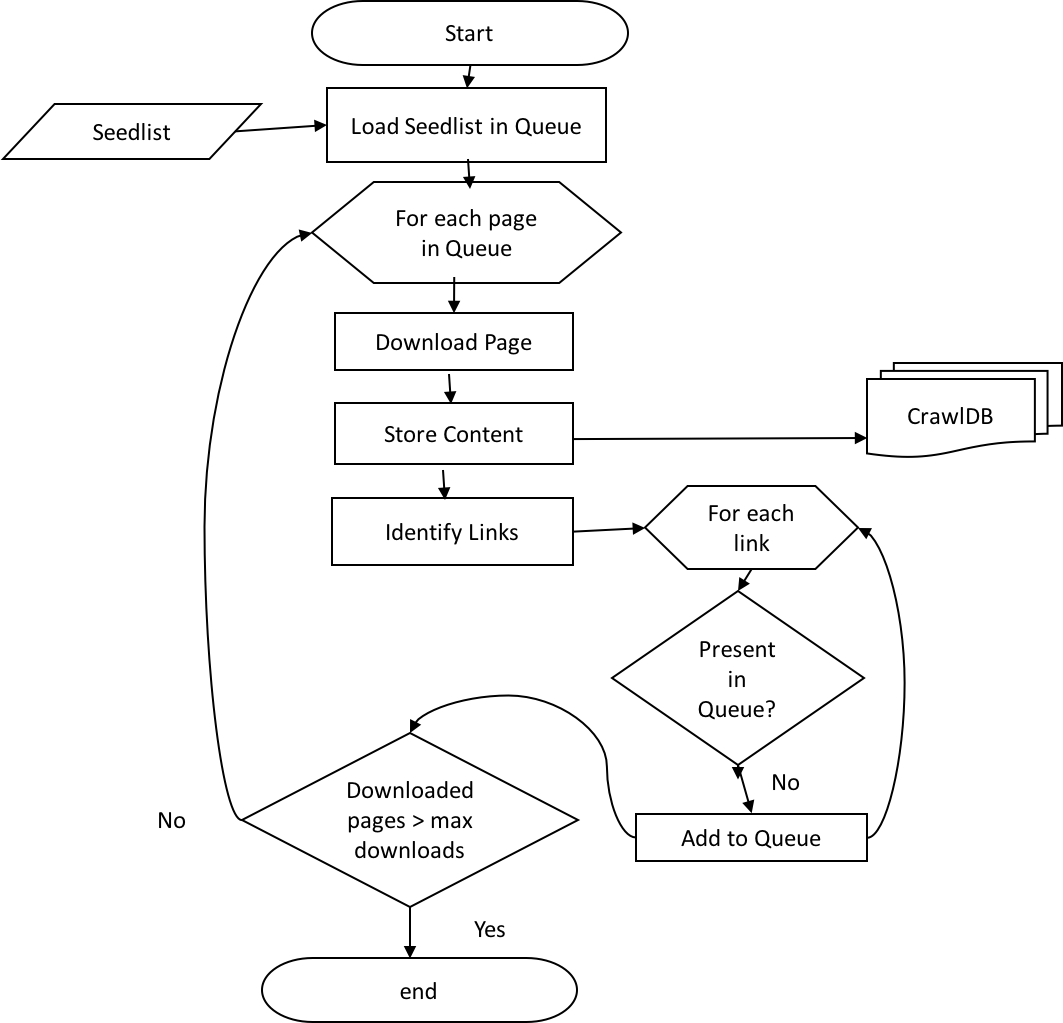
\includegraphics[width=\linewidth]{images/crawleralgo.png}}
\caption{Flowchart of crawler.}
\label{fig:crawleralgo}
\end{figure}

\subsection{Word2Vec Model Creation} \label{createmodelsection}


\subsection{Using the Word2Vec Model} \label{usemodel}




\section{Deployment}
Solution will be deployed using Ansible \cite{www-ansible} playbook. Automated deployment should happen on two or more nodes cluster. Deployment script should install all necessary software along with the project code to the cluster nodes.

\section{Benchmarking}
Solution will use collectd \cite{www-collectd} to collect statistics. Once the solution is deployed to the cluster. We should benchmark parameters like
\begin{itemize}[noitemsep]
\item cpu
\item memory
\item throughput reads/writes
\end{itemize}
Benchmarking will be done for one or more cloud providers. The deployment scripts should be agnostic to the cloud provider. 

\section{Discussion}
TBD

\section{Conclusion}

Using this wiki analysis we should be able to build a network based on wiki data.

\section{Acknowledgement}

We acknowledge our professor Gregor von Laszewski and all associate instructors for helping us and guiding us throughout this project.

\section{Appendices}
TBD

% Bibliography

\bibliography{references}
 

\end{document}
